\documentclass[a4paper]{itatnew}

\usepackage{polyglossia}
\usepackage{fontspec}
\usepackage{csquotes}
\usepackage[centertags]{amsmath}
\usepackage{amssymb}
\usepackage{bm}
\usepackage{url}
\usepackage[backend=biber,style=draft,sortlocale=en_US,bibencoding=UTF8]{biblatex}
\usepackage{hyperref}
\usepackage[inline, shortlabels]{enumitem}
\usepackage{subcaption}

\setmainfont{TeX Gyre Termes}
\setdefaultlanguage{english}

\hypersetup{
	pdfencoding=auto,
	unicode=true,
	bookmarksopen=true,
	bookmarksopenlevel=3
}

\newcommand{\name}[1]{\textbf{#1}}
\newcommand{\mathfield}{\ensuremath{\mathbb}}
\newcommand{\mathmat}{\ensuremath{\mathbf}}
\newcommand{\mathset}{\ensuremath{\mathbb}}
\newcommand{\mathspace}{\ensuremath{\mathcal}}
\newcommand{\mathvec}{\ensuremath{\bm}}

\DeclareMathOperator*{\argmin}{arg\,min}
\DeclareMathOperator*{\argmax}{arg\,max}

\title{Loss Functions for Clustering in Multi-instance Learning}
\author{Marek Dědič\inst{1,2}, Lukáš Bajer\inst{2}, Martin Holeňa\inst{3}}
\institute{Faculty of Nuclear Sciences and Physical Engineering, Czech Technical University, Trojanova 13, Prague, Czech Republic \and
Cisco Cognitive Intelligence, Karlovo náměstí 10, Prague, Czech Republic \and
Institute of Computer Science, Czech Academy of Sciences, Pod vodárenskou věží 2, Prague, Czech Republic}

\begin{document}

\twocolumn[\maketitle]

\begin{abstract}

\end{abstract}


\section{Introduction}


\section{Multi-instance Learning and Clustering}

\name{Multi-instance learning} is an approach to machine learning first described by \cite{dietterich_solving_1997}. In its original form, multi-instance learning (often referred to just as \name{MIL}) was used for \name{supervised learning}. An example of that is in the work \cite{amores_multiple_2013}. For the other class of problems solved, \name{unsupervised learning}, some prior art also exists, such as \cite{chen_contextual_2012}.

The multi-instance learning paradigm is a type of representation learning on data with some internal structure. While classical machine learning algorithms typically operate on samples represented by a vector of numbers each, MIL relaxes this requirement by representing a sample as a \name{bag} of an arbitrary number of objects. This bag is then treated as one sample -- e.g. in classification, there is a label for the whole bag.

Multi-instance learning (see \cite{dietterich_solving_1997}) in its original form is an approach to representing and solving problems where there exist samples from a space \( \mathspace{X} \) and their corresponding labels from a space \( \mathspace{Y} \) (the labels are also often called classes) and the goal is to find a mapping of samples to labels which correctly predicts the targets on the data. Unlike classical supervised learning, there is no known solution consisting of pairs of samples and labels. Instead, the samples are grouped together into so-called bags, which are defined as multisets (i.e. sets with repetition) of instances from the space \( \mathspace{X} \) such that every instance in \( \mathspace{X} \) belongs to at least one bag.

\cite{dietterich_solving_1997} provides an example of a multi-instance problem where each bag represents a key chain with some keys (instances). To solve the problem of finding which key opens a particular lock, a \enquote{proxy} MIL problem is presented -- determining which key chain opens that particular lock. This line of thinking leads to the pivotal definition of a label of the bag as a maximum over the labels of instances in said bag. In later works such as \cite{pevny_using_2017} and \cite{dedic_hierarchicke_2017}, this interpretation of MIL is abandoned in favor of a more general one. An instance is no longer viewed as having a meaning in and of itself, but only in the context of its bag. The notion of an instance-level label is dropped as in this interpretation, the bag is the atomic unit of interest. To this end, the embedded-space paradigm, described in section \ref{sec:embedded-space-paradigm}, is used in such works.

\subsection{A probabilistic formulation of multi-instance learning}\label{sec:probabilistic-formalism}
A probabilistic way of describing multi-instance learning was first introduced in \cite{pevny_using_2017} and builds on the previous work \cite{muandet_learning_2012}.

Let for the space \( \mathspace{X} \) exist a measurable space \( \left( \mathspace{X}, \mathspace{A} \right) \), where \( \mathspace{A} \) is a \( \sigma \)-algebra of \( \mathspace{X} \). Let \( \mathcal{P}^\mathspace{X} \) denote the set of all probability measures on \( \left( \mathspace{X}, \mathspace{A} \right) \). A bag \( B \) is viewed as a set of realizations of a particular probability distribution \( P \in \mathcal{P}^\mathspace{X} \), that is
\[ B = \left\{ x_i \middle| x_i \sim P, i \in \left\{ 1, \dots, m \right\}, m \in \mathfield{N} \right\} \]
A core assumption of this formalism is that \( P = P \left( P_B, y_B \right) \) where \( P_B \) is the probability distribution of instances in the bag \( B \) and \( y_B \) is the label assigned to \( B \). That is, the probability distribution of the bag is dependent on its assigned label.

\subsection{Embedded-space paradigm for solving multi-instance problems}\label{sec:embedded-space-paradigm}

While it is possible to use several approaches to solving multi-instance problems, in this work, the embedded-space paradigm was used. For an overview of the other paradigms, see \cite{dedic_optimalization_2020}.

In the embedded space paradigm, labels are only defined on the level of bags. In order for these bag labels to be learned, an embedding function of the form \( \phi : \mathspace{B} \to \bar{\mathspace{X}} \) must be defined, where \( \bar{\mathspace{X}} \) is a latent space, which may or may not be identical to \( \mathspace{X} \). Using this function, each bag can be represented by an object \( \phi \left( B \right) \in \bar{\mathspace{X}} \), which makes it possible to use any off-the-shelf supervised learning algorithm acting on \( \bar{\mathspace{X}} \). Among the simplest embedding functions are e.g. element-wise minimum, maximum and mean. A more complicated embedding function may for example apply a neural network to each instance of the bag and subsequently pool the instances using one of the aforementioned functions.

\cite{pevny_nested_2020} and \cite{dedic_hierarchicke_2017} present an approach to learning to classify HTTP traffic by utilizing sets of URLs. Neural networks are used to transform both instance-level and bag-level representations. The model is as follows. A deep neural network \( f_I : \mathspace{X}_1 \to \mathspace{X}_2 \) is used to transform each instance \( x \in B \). An aggregation function is then used, being of the form
\[ g: \mathcal{P}^M \left( \mathspace{X}_2 \right) \to \bar{\mathspace{X}}_1 \ \]
Finally, a second deep neural network \( f_B : \bar{\mathspace{X}}_1 \to \bar{\mathspace{X}}_2 \) is used to transform the representation of each bag. Combining these functions gives the embedding function
\[ \phi \left( B \right) = f_B \left( g \left( \left\{ f_I \left( \mathvec{x} \right) \middle| \mathvec{x} \in B \right\} \right) \right) \]
The functions \( f_I \) and \( f_B \) are realized by a deep neural network using ReLU as its activation function. The aggregation \( g \) is realized as an element-wise mean or maximum of all the vectors.

The structure of the data is highly exploited using the embedded-space paradigm. The approach is innovative in that it uses multiple layers of MIL nested in each other -- that is the instances of a bag do not necessarily need to be feature vectors, but can be bag in themselves. The HTTP traffic of a particular client is therefore represented as a bag of all second-level domains the client has exchanged datagrams with. Each second-level domain is then represented as a bag of individual URLs which the client has connected to. Individual URLs are then split into 3 part, domain, path and query, and each part is represented as a bag of tokens, which can then be broken down eve further. The model is shown in figure \ref{fig:HTTP-paper}. In the end, the model consists of 5 nested MIL problems.

\begin{figure*}
	\centering
	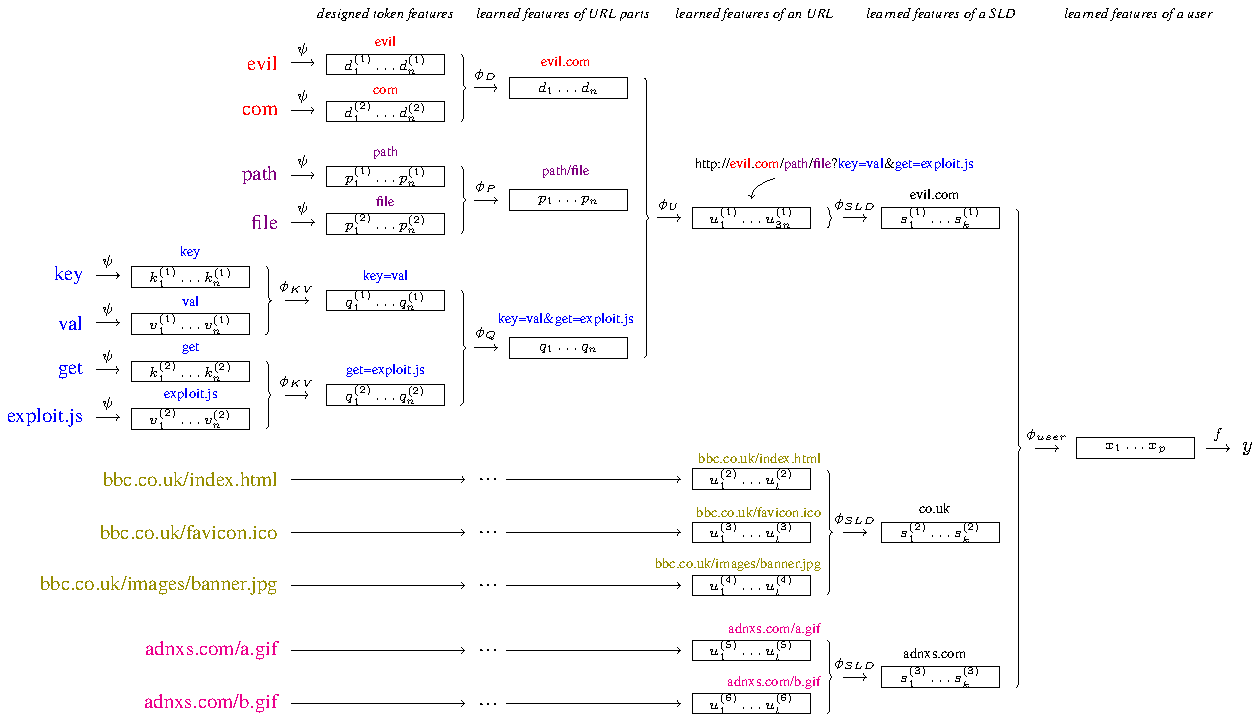
\includegraphics[width=\textwidth]{images/HTTP-paper/HTTP-paper.pdf}
	\caption{Hierarchical model of the network traffic of a single computer. The computer is modelled by a set of remote servers and each remote server is modelled by a set of messages (connections) from the given computer to it. Figure from \cite{pevny_nested_2020}.}\label{fig:HTTP-paper}
\end{figure*}

An added benefit of MIL is also in its relatively easy explainability and interpretability. \cite{pevny_nested_2020} present a way to extract indicators of compromise and explain the decision using the learned MIL model.

\subsection{Clustering}

Clustering is a prime example of a problem typically associated with unsupervised learning.\footnote{In this work, both unsupervised and supervised approaches to clustering are explored.} \cite{xu_comprehensive_2015} even call clustering the most important question of unsupervised learning. The problem at hand, however, is not one of clustering ordinary number vectors in a linear space. Instead, a clustering of objects represented by bags is explored, as that is the problem solved for datasets introduced later in section \ref{sec:experimental-comparison}. While \cite{wang_solving_2000} present a clustering of bags using a modified Hausdorff distance on bags and \cite{kohout_network_2018} present a clustering of network traffic fingerprints using maximum mean discrepancy, this approach was not chosen in this work. Among the main reasons for this choice is the prohibitively high computational complexity of bag-space paradigm approaches on large datasets and the opportunity to utilize the representations previously introduced for the particular datasets in \cite{dedic_hierarchicke_2017} and \cite{pevny_nested_2020}.

An approach based on the embedded-space paradigm (see section \ref{sec:embedded-space-paradigm}) for MIL was chosen. In order to utilize the structure of the data, a MIL model is used to represent each bag in the latent space \( \bar{\mathspace{X}} \). This presents the issue of how to train the embedding function \( \phi \) -- MIL as presented previously is a supervised algorithm, whereas clustering is a typically unsupervised problem.

The embedding function \( \phi \) from section \ref{sec:embedded-space-paradigm} is actually of the form
\[ \phi = \phi \left( B, \mathvec{\theta} \right) \qquad \text{where} \quad B \in \mathspace{B} \]
where \( \mathvec{\theta} \) are the parameters of the embedding, typically learned during the training phase. In the context of clustering, these parameters still need to be learned over the training phase somehow. This in and of itself presents another challenge though -- off-the-shelf algorithms typically work in some kind of constant Hilbert space, whereas in this example, the latent space needs to change over the learning period. As is the case for MIL itself, end-to-end learning was chosen as an approach to solve both of these problems. A clustering-loss function \( L_C \) is chosen such that
\[ L_C: \mathcal{P}^M \left( \bar{\mathspace{X}} \right) \to \mathfield{R} \]
Given such clustering-loss function, an actual loss for the embedding model \( \phi \) and its parameters \( \mathvec{\theta} \) can be computed as
\[ L \left( \phi, \mathvec{\theta} \right) = L_C \left( \left\{ \phi \left( B, \mathvec{\theta} \right) \middle| B \in \mathspace{B} \right\} \right) \]
If the cluster-loss \( L_C \) is chosen correctly, minimizing \( L \) over the learning period will yield a latent space \( \bar{\mathspace{X}} \) in which the bags are already naturally clustered according to the design of the cluster-loss function. Applying any off-the-shelf clustering algorithm on \( \bar{\mathspace{X}} \) will then give good results. How to choose the cluster-loss function \( L_C \) is the focus of section \ref{sec:loss-functions}.

\subsection{Clustering evaluation metrics}\label{sec:clustering-metrics}

\cite{xu_comprehensive_2015} present different clustering performance metrics. In this work, several metrics are used. The primary metrics are based on the Silhouette coefficient, the secondary ones on the kNN algorithm (see \cite{dasarathy_nearest_1991}). The metrics are somewhat different to the ones traditionally used in evaluating clustering methods as all the datasets used in this work are originally classification datasets and therefore have classes available. Each class can then be viewed as a cluster target and the learned clustering evaluated against these targets.

The first two metrics measure the \name{homogeneity} (that is the property of instances of one cluster being close to one another) and \name{separation} (that is the property of instances of different clusters being far apart) of clusters (see \cite{everitt_cluster_2001}). To measure the homogeneity of a cluster, the average distance between items in a cluster is measured and averaged over all clusters, giving the following metric for items \( x_j \) in clusters \( C_i \) (defined by the classes in the data):
\[ \mu \left( C_i \right) = \frac{1}{\left\lvert C_i \right\rvert} \sum_{x_j \in C_i} x_j \]
\[ \mathrm{homo} \left( C_1, \dots, C_n \right) = \frac{1}{n} \sum_{i = 1}^n \sum_{x_j \in C_i} \left\lVert x_j - \mu \left( C_i \right) \right\rVert \]

To measure the separation of clusters, the average distance between cluster centres was taken:
\[ \mathrm{sep} \left( C_1, \dots, C_n \right) = \frac{2}{n \left( n - 1 \right)} \sum_{\substack{i, j \in \hat{n} \\ i < j }} \left\lVert \mu \left( C_i \right) - \mu \left( C_j \right) \right\rVert \]

The final primary metric is akin to the Silhouette coefficient:
\[ \mathrm{silhouette} \left( C_1, \dots, C_n \right) = \frac{\mathrm{sep} \left( C_1, \dots, C_n \right)}{\mathrm{homo} \left( C_1, \dots, C_n \right)} \]

For the secondary metrics, the kNN algorithm is used and its accuracy (i.e. the fraction of correctly classified samples) measured. The kNN algorithm was seeded with the training data and its accuracy assessed on the testing data. This was done over the learning period, giving the first metric. Secondly, on the final model, the kNN classifier has been seeded with different amount of data and its performance measured (typically, this data is called the training data of the kNN classifier, in this work, however, it is referred to as \name{seed data} to avoid confusion with the data used to train the embedding). This gives a view into the robustness of the clustering, as high-quality embeddings would need only a small amount of seed data points to reach relatively high accuracy. For this last measure, the kNN algorithm was run thrice and the results averaged to compensate for high dependence on the particular seed points chosen if there is only a few of them.

\section{Investigated Loss Functions}\label{sec:loss-functions}

In section \ref{sec:clustering-metrics}, a method for learning a representation \( \phi \) was shown. In order to learn the parameters of the representation, a clustering-loss function is required in the form
\[ L_C : \mathcal{P}^M \left( \bar{\mathspace{X}} \right) \to \mathfield{R} \]
In this section, three ways of constructing such a clustering-loss function are explored. First, an unsupervised method constructing a clustering loss-function is presented, followed by two supervised methods.


\subsection{Contrastive Predictive Coding}
Contrastive predictive coding (also referred to as \name{CPC}) is a technique first introduced by \cite{oord_representation_2019}. The method builds the model on the ideas from predictive coding (see \cite{elias_predictive_1955}), a technique from information theory. CPC is an approach to representing time series by modelling future data from the past. In order to do that, the model learns high-level representations of the data and discards noise in the data. The further in future the model predicts, the less shared information is available and thus the global structure needs to be inferred better.

The core idea taken from CPC to this work is that of a loss function called the InfoNCE in the prior art. Given a set \( \mathset{X} = \left\{ x_1, \dots, x_N \right\} \) containing one positive sample from \( p \left( x_{t + k} \middle| c_t \right) \) and \( N - 1 \) negative samples from \( p \left( x_{t + k} \right) \) where \( c_t \) is a context provided by an autoregressive model summarizing latent representations up to the time point \( t \), the InfoNCE loss is as follows:
\[ - \underset{\mathset{X}}{\mathbb{E}} \left[ \log f_k \left( x_{t + k}, c_t \right) - \log \sum_{x_j \in \mathset{X}} f_k \left( x_j, c_t \right) \right] \]

The actual application is based on the following idea. If a bag is split into two parts, it is reasonable to expect that the representations of these two parts would be close to one another. On the other hand, if a random bag were to be drawn from the data (as a \textit{simple random sample with replacement}), it is reasonable to expect it to be relatively far from any actual bag present in the data. These assumptions can be proven correct by using the probabilistic formalism for MIL (see section \ref{sec:probabilistic-formalism}). Given that each bag \( B_k \) is viewed as a set of realizations of a probability distribution \( P_k \in \mathcal{P}^\mathspace{X} \), it follows that the two parts of the bag, \( B_k^{(1)} \) and \( B_k^{(2)} \), are sets of realizations from the same distribution \( P_k \) and therefore should be statistically indistinguishable. On the other hand, a randomly sampled bag \( B'_j \) does not share the same probability distribution.
Using these assumptions, the following clustering loss is constructed:
\[ \forall j \; B'_j \text{ is a bag of randomly sampled instances from } \mathspace{X} \]
\begin{align*}
	L_\mathrm{CPC} = &\log \left\lVert \phi \left( B_k^{(1)} \right) - \phi \left( B_k^{(2)} \right) \right\rVert^2 \\
	- &\log \sum_{j = 1}^K \left\lVert \phi \left( B_k^{(1)} \right) - \phi \left( B'_j \right) \right\rVert^2
\end{align*}
The first term of the loss function depicts the notion that the representations of the two parts of the bag should be close to one another and corresponds to the first term of InfoNCE, which maximizes the prediction of a matching future sample from the current context. The second term depicts the notion that a random bag should be far from all the bags\footnote{On the off-chance a random bag would be close to \( B_k^{(1)} \), this would be outweighed by the other terms.} and corresponds to the second term of InfoNCE, which minimizes the prediction of a random sample from the current context. Choosing to only use the first part of the bag in the second term has no effect as the two parts are chosen randomly. The value \( K \in \mathfield{N} \) is a hyper-parameter of this method.

This method can be further modified to make it less computationally complex. In order to not have to draw a lot of random bags, it can be reasonably expected that, on average, the representations of two parts of two mismatched bags \( B_{k_1}^{(1)} \) and \( B_{k_2}^{(2)} \) should be far apart. The matrix \( \mathmat{D} \) is constructed as
\begin{equation}\label{eq:bag-distance-matrix}
	\mathmat{D}_{ij} = \left\lVert \phi \left( B_i^{(1)} \right) - \phi \left( B_j^{(2)} \right) \right\rVert_2^2
\end{equation}
The distances of the corresponding halves are found on the diagonal of \( \mathmat{D} \), whereas the distances of mismatched halves are in the rest of the matrix. Under this assumption the final loss for the CPC method is
\[ L_\mathrm{CPC} = \frac{1}{n} \sum_{i = 1}^n \left( \log \left( \mathmat{D}_{ii} \right) - \log \sum_{\substack{j = 1 \\ j \neq i}}^n \mathmat{D}_{ij} \right) \]
where \( n \) is the number of bags.

\subsection{Triplet Loss}

The performance of the \( k \)-nearest neighbour algorithm depends heavily on the distance metric used. Typically, the Euclidean distance is used. However, ideally, the metric would adapt to the problem at hand. \cite{weinberger_distance_2006} present a way to learn a Mahalanobis distance metric for kNN such that it has the \textit{homogeneity} and \textit{separation} properties of clustering. This distance metric, the description of which follows, has been utilized in this work as the basis for the desired loss function \( L_C \).

Let \( \left\{ \left( \mathvec{x}_i, y_i \right) \right\}_{i = 1}^n \) be a training dataset with \( \mathvec{x}_i \in \mathfield{R}^d \) and \( y_i \) discrete class labels. The goal is to learn a linear transformation
\[ \mathvec{L} : \mathfield{R}^d \to \mathfield{R}^d \]
This linear transformation is then used to compute squared distances as
\[ \mathcal{D} \left( \mathvec{x}_i, \mathvec{x}_j \right) = \left\lVert \mathvec{L} \left( \mathvec{x}_i - \mathvec{x}_j \right) \right\rVert_2^2 \]

A helper matrix \( \mathmat{y} \) is used such that
\[ \mathmat{y}_{ij} = \begin{cases}
	0 &\text{for} \quad y_i \neq y_j \\
	1 &\text{for} \quad y_i = y_j \\
\end{cases} \]
In addition to this, for each input \( \mathvec{x}_i \), \( k \) target neighbours are defined that are supposed to be close to \( \mathvec{x}_i \). Euclidean distance may be used to find the target neighbours. A matrix \( \mathmat{\eta} \) is used to indicate target neighbours where \( \mathmat{\eta}_{ij} = 1 \) when \( \mathvec{x}_j \) is a target neighbour of \( \mathvec{x}_i \) and \( 0 \) otherwise.

The cost function features two competing terms. The first term depicts the notion that an input should be close to its target neighbours. The second term depicts the notion that inputs of a different class should be far from one another. The loss is of the form
\begin{align*}
	&\sum_{i, j = 1}^n \mathmat{\eta}_{ij} \left\lVert \mathvec{L} \left( \mathvec{x}_i - \mathvec{x}_j \right) \right\rVert_2^2 + \\
	&+ c \sum_{i, j, l = 1}^n \mathmat{\eta}_{ij} \left( 1 - \mathmat{y}_{il} \right) \left\{ \left\lVert \mathvec{L} \left( \mathvec{x}_i - \mathvec{x}_l \right) \right\rVert_2^2 - \left\lVert \mathvec{L} \left( \mathvec{x}_i - \mathvec{x}_j \right) \right\rVert_2^2 \right\}_+
\end{align*}
where \( c > 0 \) is a hyper-parameter of this method and \( \left\{ \cdot \right\}_+ \) is the hinge loss.

In the original work, this loss is then reformulated as an instance of semidefinite programming, however, this has not been pursued in this work. Instead, to adapt the original method, the definitions need to be modified to leverage the bagging of the data. The matrix \( \mathmat{y} \) is defined in the same way, only with labels on the level of bags. The value \( \mathmat{\eta}_{ij} = 1 \) iff bag \( B_j \) is a target neighbour for the bag \( B_i \). Then, using the matrix \( \mathmat{D} \) defined in equation \ref{eq:bag-distance-matrix}, the loss function can be expressed as

\[ L_\mathrm{triplet} = \sum_{ij} \eta_{ij} D_{ij} + c \sum_{ijl} \eta_{ij} \left( 1 - y_{il} \right) \left\{ D_{il} - D_{ij} \right\}_+ \]

where \( c > 0 \) is a hyper-parameter of the method. Although \cite{weinberger_distance_2006} suggest finding \( \mathmat{\eta} \) as the \( k \)-nearest neighbours of a data point, in this work, the loss has been simplified by setting \( \mathmat{\eta}_{ij} = \mathmat{y}_{ij} \).

\subsection{Magnet Loss}

\section{Experimental Comparison}\label{sec:experimental-comparison}


\subsection{Datasets}


\subsection{Experimental Design}


\subsection{Comparison Results}


\section{Conclusion}


\subsection*{Acknowledgement}

The research reported in this paper has been supported by the Czech Science Foundation (GAČR) grant 18-18080S.

\printbibliography
\end{document}
